%%%%%%%%%%%%%%%%%%%% book.tex %%%%%%%%%%%%%%%%%%%%%%%%%%%%%
%
% sample root file for the chapters of your "monograph"
%
% Use this file as a template for your own input.
%
%%%%%%%%%%%%%%%% Springer-Verlag %%%%%%%%%%%%%%%%%%%%%%%%%%


% RECOMMENDED %%%%%%%%%%%%%%%%%%%%%%%%%%%%%%%%%%%%%%%%%%%%%%%%%%%
\documentclass[pdftex,12pt, oneside]{article}

% choose options for [] as required from the list
% in the Reference Guide, Sect. 2.2
%\usepackage[paperwidth=8.5in, paperheight=13in]{geometry} % Folio
\usepackage[paperwidth=8.27in, paperheight=11.69in]{geometry} % A4

\usepackage{makeidx}         % allows index generation
\usepackage{graphicx}        % standard LaTeX graphics tool
                             % when including figure files
%\usepackage{multicol}        % used for the two-column index
\usepackage[bottom]{footmisc}% places footnotes at page bottom
\usepackage[bahasa]{babel}
\usepackage{enumerate}
\usepackage{paralist}
\usepackage{float}
\usepackage{gensymb}  
\usepackage{listings}
\usepackage{hyperref}
%\usepackage{siunitx}
% etc.
% see the list of further useful packages
% in the Reference Guide, Sects. 2.3, 3.1-3.3
\renewcommand{\baselinestretch}{1.5}

\newcommand{\HRule}{\rule{\linewidth}{0.5mm}}

%\makeindex             % used for the subject index
                       % please use the style svind.ist with
                       % your makeindex program


%%%%%%%%%%%%%%%%%%%%%%%%%%%%%%%%%%%%%%%%%%%%%%%%%%%%%%%%%%%%%%%%%%%%%

\begin{document}

%\input{./01.title.tex}
\begin{center}
{\large STUDI KELAYAKAN PENDAHULUAN PEMBANGUNAN SISTEM OTENTIKASI DI BADAN PENGELOLAAN PENDAPATAN, KEUANGAN DAN ASET DAERAH KABUPATEN BREBES}
\\[1cm]
15 Februari 2019\\
Priyanto Tamami, S.Kom.
\end{center}

\section{PENENTUAN MASALAH DAN PELUANG YANG DITUJU SISTEM}

\subsection{Penentuan Masalah}

Sudah lama sejak penerapan Undang Undang Nomor 28 Tahun 2009 tentang Pajak Daerah dan Retribusi daerah, beberapa kewenangan atas jenis pajak yang sebelumnya dikelola oleh Pemerintah Pusat, dengan Undang-Undang ini kewenangannya dilimpahkan ke Pemerintah Daerah dengan tujuan memberikan kekuatan dan kemandirian daerah dengan penopang yang bersumber dari Pendapatan Asli Daerah.

Beberapa ketentuan mengenai Retribusi pun diatur dalam Undang Undang Nomor 28 Tahun 2009 yang dikenal dengan Undang Undang PDRD (Pajak Daerah dan Retribusi Daerah) ini.

Dengan perluasan jenis pajak yang dilimpahkan ke Pemerintah Daerah, terkhusus Pemerintah Kabupaten / Kota, maka data yang perlu dikelola pun semakin bertambah, terlebih saat melakukan pengelolaan Pajak Bumi dan Bangunan Perdesaan dan Perkotaan.

Pada pelimpahan jenis pajak Pajak Bumi dan Bangunan Perdesaan dan Perkotaan, Pemerintah Kabupaten Brebes menerima data sejumlah kurang lebih 1 juta objek pajak. Penyerahan jenis pajak ini tidak hanya data, melainkan aplikasi untuk pengelolaannya pun dilimpahkan juga, sehingga Pemerintah Daerah diharapkan dapat langsung melakukan kegiatan operasionalnya pada Tahun pelimpahan terjadi.

Serupa dengan jenis pajak Pajak Bumi dan Bangunan Perdesaan dan Perkotaan, jenis pajak yang lain pun dituntut untuk lebih tertib administrasi dalam pengelolaannya sehingga penggunaan aplikasi pun diterapkan untuk mempermudah prosesnya.

Untuk jenis pajak selain Pajak Bumi dan Bangunan Perdesaan dan Perkotaan sudah beberapa kali terjadi perubahan implementasi dalam penggunaan aplikasi atau sistem informasi, perubahan ini terjadi karena adanya perubahan struktur pada Badan atau Dinas yang melakukan pengelolaan Pajak Daerah. 

Imbas yang terjadi karena perubahan implementasi sistem atau aplikasi yang digunakan ini adalah perlunya adaptasi dan pelatihan terhadap penggunaan aplikasi tersebut sehingga terkadang mengganggu proses pelayanan.

Selain perubahan dari sistem informasi atau aplikasi untuk pengelolaan Pajak Daerah, pada Badan Pengelolaan Pendapatan, Keuangan dan Aset Daerah Kabupaten Brebes pun menggunakan banyak aplikasi yang berbeda-beda, sehingga masing-masing pengguna terkadang akan memiliki beberapa akun yang berbeda untuk masing-masing aplikasi atau sistem yang digunakan sesuai dengan tugas dan fungsinya masing-masing.

Seiring berjalannya waktu, kebutuhan akan data yang disimpan dan dikelola tentunya akan semakin bertambah, untuk itu akan diperlukan beberapa aplikasi lagi yang semakin berkembang menyesuaikan kebutuhannya.

Dari hal tersebut, tentunya masing-masing administrator sistem pun akan membuat akun untuk masing-masing pengguna yang jelas akan banyak sekali redundansi data.

\subsection{Peluang Yang Dituju}

Dari kondisi tersebut di atas diperlukan sebuah aplikasi yang mampu memberikan layanan otentikasi dan otorisasi tunggal, dimana masing-masing pengguna nantinya hanya cukup membutuhkan sebuah akun dan \textit{password} untuk melakukan akses data ke berbagai aplikasi yang ada, sesuai dengan tugas dan fungsi serta kewenangannya masing-masing.

Mengacu kepada Konsep OAuth2 yang dijelaskan pada IETF dengan nomor RFC 6749, bahwa kerangka kerja OAuth2 mampu memberikan otentikasi dan otorisasi terhadap pengguna dalam melakukan akses ke \textit{resource server}.

Nantinya akan ada 4 (empat) bagian yang berperan dalam implementasi ini, bagian tersebut adalah seperti berikut :

\begin{enumerate}

\item \textit{Authorization Server} yang berfungsi untuk melakukan otentikasi dan otorisasi terhadap pengguna, nantinya \textit{Authorization Server} akan memberikan sebuah token akses ke Aplikasi Klien setelah melakukan otentikasi terhadap pengguna.

\item \textit{Resource Server} yang nantinya berperan untuk memberikan data yang dibutuhkan atau sebagai \textit{back-end} dari aplikasi klien dalam mengelola data, nantinya \textit{Resource Server} ini akan melakukan akses langsung ke sistem basis data tempat sumber data berada. \textit{Resource Server} pun akan dilindungi oleh mekanisme akses data terbatas dimana otentikasi yang diberikan kepada pengguna akan difilter dan di verifikasi oleh \textit{Resource Server} yang dikomunikasikan dengan \textit{Authorization Server}.

\item Aplikasi Klien yang dibangun untuk melakukan akses terhadap  \textit{Resource Server} dengan menggunakan konsep otorisasi yang diberikan oleh \textit{Authorization Server} berupa sebuah token dari hasil otentikasi Pengguna di \textit{Authorization Server}, dimana pertukaran data atau informasi antara Aplikasi klien dengan \textit{Resource Server} akan selalu mengirimkan sebuah token sebagai bahan otentikasi. Aplikasi Klien ini tidak terbatas kepada aplikasi \textit{desktop}, atau \textit{mobile}, atau \textit{web}, melainkan aplikasi yang di eksekusi di peladen pun apabila memanfaatkan \textit{Resource Server} yang terhubung dengan \textit{Authentication Server} ini akan dianggap sebagai Aplikasi Klien.

\item Pengguna, ini adalah entitas yang memiliki hak akses ke \textit{Resource Server} untuk melakukan manipulasi atau akses data sesuai dengan kewenangan yang diberikan.
\end{enumerate}

Studi kelayakan ini akan menitikberatkan pada pembentukan \textit{Authorization Server} sebagai sarana untuk melakukan otentikasi dan otorisasi sistem, sehingga diharapkan seluruh sistem yang dibangun berikutnya akan mengacu pada penggunaan \textit{Authorization Server} ini untuk melakukan otentikasi dan otorisasi.

Tidak terbatas pada aplikasi yang akan dibangun yang bersifat baru sesuai kebutuhan organisasi, namun aplikasi-aplikasi atau sistem yang sifatnya adalah migrasi dari sistem lama, diharapkan akan menggunakan \textit{Authorization Server} ini sebagai sarana melakukan otorisasi dan otentikasi.

\section{PEMBENTUKAN SASARAN SISTEM BARU SECARA KESELURUHAN}

Sasaran dari sistem baru ini secara keseluruhan adalah dapat melakukan otentikasi dan otorisasi terhadap pengguna dan sistem informasi atau aplikasi yang digunakan oleh pengguna.

Pada bagian otentikasinya, pengguna nantinya akan datang dari sebuah aplikasi atau langsung membuka halaman otentikasi, dalam hal ini adalah halaman \textit{login} yang kemudian mengisikan \textit{username} dan \textit{password}, kemudian pengguna akan mendapatkan sebuah token yang dapat digunakan untuk melakukan akses ke beberapa aplikasi yang sudah mendukung dan terhubung dengan sistem \textit{Authorization Server}.

Alur secara umum dapat diilustrasikan seperti pada gambar \ref{fig:flow-oauth} berikut ini :

\begin{figure}[H]
	\centering
	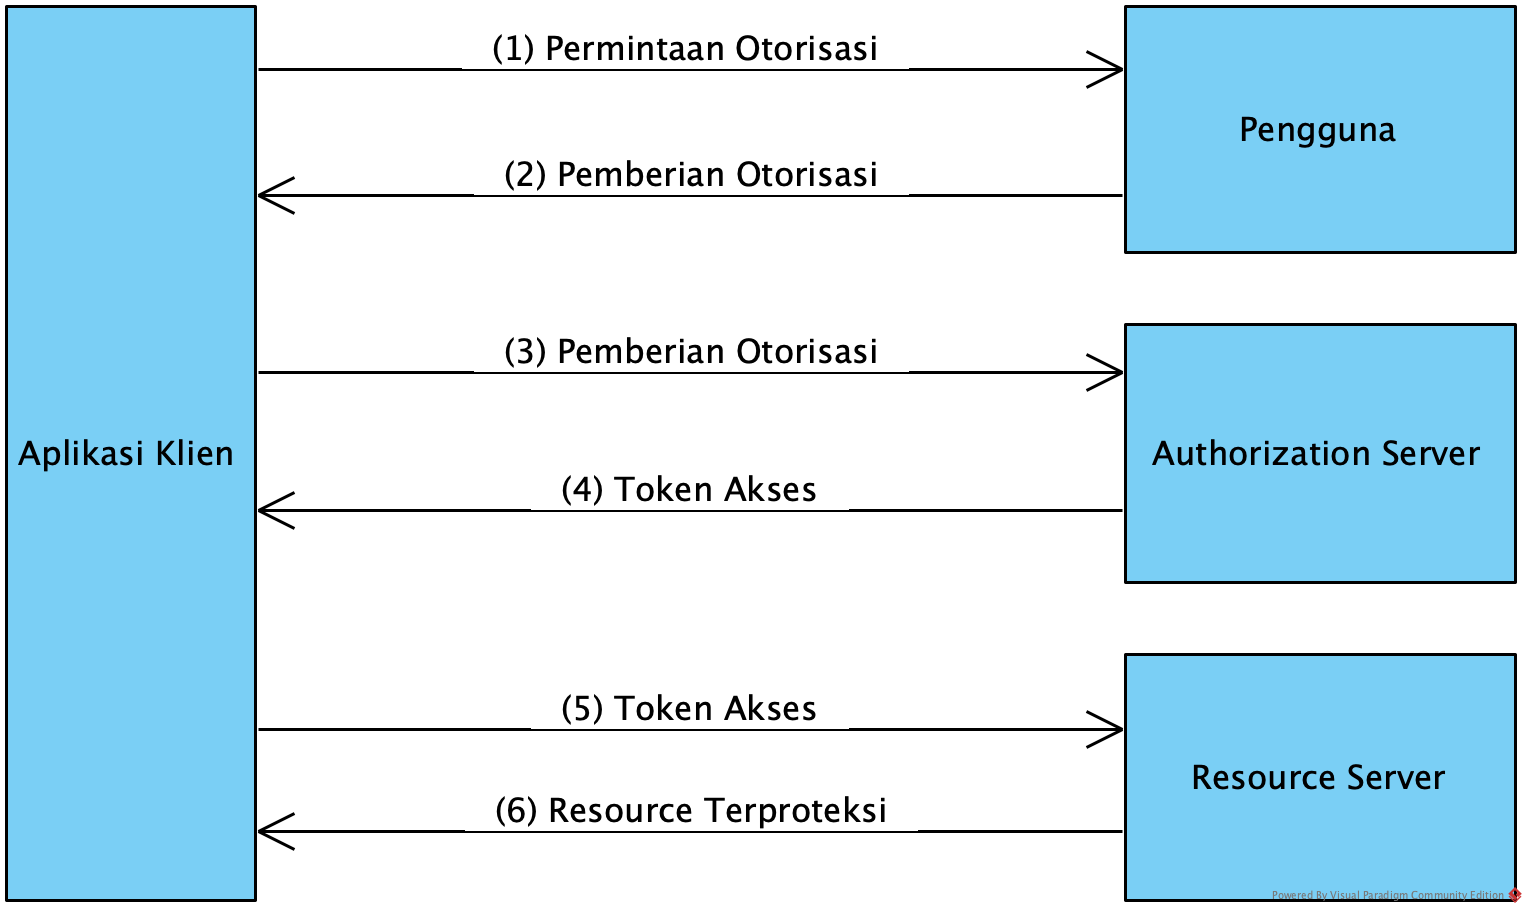
\includegraphics[width=1\textwidth]{./resources/flow-oauth-protocol}
	\caption{Diagram Alur Otorisasi Secara Umum}
	\label{fig:flow-oauth}
\end{figure}

Langkah dari gambar \ref{fig:flow-oauth} tersebut adalah seperti berikut, dengan urutan angka pada diagram menunjukkan proses atau tahapan yang terjadi :

\begin{enumerate}
	
	\item Aplikasi Klien akan mengirimkan permintaan otorisasi dari pengguna yang biasanya berbentuk pasangan \textit{username} dan \textit{password}. Permintaan otorisasi ini bisa dilakukan langsung kepada pengguna dari Aplikasi Klien, atau diserahkan ke \textit{Authorization Server} sebagai aplikasi penghubung.

	\item Aplikasi Klien akan menerima otorisasi berupa pasangan \textit{username} dan \textit{password} dari Pengguna yang tentunya dengan kewenangan yang telah diberikan. Prosesnya akan menggunakan salah satu dari 4 (empat) bentuk otorisasi yang ada pada protokol OAuth 2. Tipe atau bentuk otorisasinya sudah disepakati bersama antara Aplikasi Klien dengan \textit{Authorization Server}.

	\item Aplikasi Klien melakukan permintaan Token Akses ke \textit{Authorization Server} dengan membawa informasi otorisasi dari Pengguna.
	
	\item \textit{Authentication Server} memastikan bahwa informasi otorisasi yang dikirimkan sesuai dengan yang terdaftar, bila informasinya benar, maka akan diberikan Token Akses, namun bila tidak terdaftar atau informasinya salah, maka akan mengirimkan informasi bahwa pengguna tidak terdaftar atau tidak memiliki hak atau kewenangan.
	
	\item Aplikasi Klien akan melakukan permintaan data ke \textit{Resource Server} dengan menyertakan Token Akses sebagai pengenal otorisasinya.
	
	\item Kemudian \textit{Resource Server} akan melakukan verifikasi terhadap Token Akses yang telah diterima dari Aplikasi Klien, apabila Token Akses benar, maka \textit{Resource Server} akan memberikan data atau informasi yang diminta.
	
\end{enumerate}

Cara yang dianjurkan untuk digunakan saat Aplikasi Klien melakukan permintaan data otentikasi dari Pengguna (sebagaimana pada langkah 1 dan 2), adalah menggunakan \textit{Authorization Server} sebagai perantara. Hal ini diharapkan menghilangkan kecurigaan dari sisi Pengguna bahwa \textit{username} dan \textit{password} yang diberikan tidak disimpan atau disalahgunakan oleh Aplikasi Klien untuk melakukan hal yang tidak diketahui oleh Pengguna, di sisi lain pun menyederhanakan pembangunan sebuah Aplikasi Klien tanpa perlu membuat sebuah halaman otentikasi lagi, karena halaman ini sudah disediakan oleh \textit{Authorization Server}.

Pada tahap otorisasi nantinya akan ada beberapa jenis alur yang dapat dapat digunakan yang biasanya akan melihat dengan teknik apa Aplikasi Klien dibangun. Berikut adalah spesifikasi yang didefinisikan dalam Dokumen IETF RFC 6749 :

\begin{enumerate}

	\item Authorization Code.
	
	\textit{Authorization code} atau kode otorisasi didapat dari \textit{Authorization Server} yang diposisikan sebagai penghubung antara Aplikasi Klien dan \textit{Resource Server}. Aplikasi Klien tidak meminta informasi \textit{username} dan \textit{password} secara langsung dari Pengguna, melainkan Pengguna akan diarahkan ke \textit{Authorization Server} untuk melakukan \textit{login}, setelah berhasil maka Pengguna akan diarahkan kembali ke Aplikasi Klien beserta kode otorisasi.
	
	Karena Pengguna melakukan otentikasi langsung ke \textit{Authorization Server}, informasi rahasia seperti \textit{username} dan \textit{password} tidak perlu diketahui oleh Aplikasi Klien.
	
	Skema atau spesifikasi ini memiliki keamanan yang cukup untuk melakukan otentikasi terhadap Aplikasi Klien, termasuk pengiriman Token Akses yang langsung ke Aplikasi Klien yang berpotensi terhadap bocornya Token Akses ke pihak lain.
	
	Skema atau spesifikasi ini biasanya diterapkan pada Aplikasi Klien yang mampu untuk menyimpan kode otorisasi dengan aman, misalnya seperti aplikasi server yang dibangun dengan PHP, Java, NodeJS, dan sebagainya, atau aplikasi berbasis \textit{Desktop} atau \textit{Mobile} yang dapat di\textit{compile}.
	
	\item User Password
	
	Pada spesifikasi ini, \textit{username} dan \textit{password} dapat langsung digunakan untuk mendapatkan Token Akses dari \textit{Authorization server}. Karena hal ini tentunya Pengguna memiliki kepercayaan penuh terhadap Aplikasi Klien yang digunakannya. Yang biasanya terjadi adalah aplikasi klien \textit{mobile}, \textit{desktop} atau \textit{web} yang digunakan dibuat sendiri, sehingga kita sebagai pengguna meyakini bahwa aplikasi tersebut tidak akan berbuat curang.
	
	Meskipun pada spesifikasi ini Aplikasi Klien menerima \textit{username} dan \textit{password} dari pengguna untuk kemudian di otentikasi oleh \textit{Authorization Server} namun tetap saat kondisi \textit{username} dan \textit{password} sudah benar, Aplikasi Klien akan menerima Token Akses untuk melakukan akses ke \textit{Resource Server}.
	
	\item Implicit
	
	Spesifikasi alur \textit{implicit} ini menyederhanakan alur yang digunakan oleh spesifikasi \textit{Authorization Code} yang biasanya diimplementasikan bagi Aplikasi Klien yang dibangun bahasa interpreter seperti JavaScript.
	
	Perbedaannya dengan spesifikasi \textit{Authorization Code} adalah bahwa \textit{Authorization Server} tidak perlu memberikan kode otorisasi ke Aplikasi Klien, melainkan langsung diberikan Token Akses secara langsung.
	
	Ketika memberikan Token Akses ke aplikasi klien, \textit{Authorization Server} tidak melakukan otentikasi terhadap Aplikasi Klien, dimana pada beberapa implementasi, identitas Aplikasi Klien diverifikasi melalui alamat \textit{redirection} URI tempat dikirimnya Token Akses. Token Akses sendiri nantinya dapat dilihat oleh Pengguna atau aplikasi lain yang memiliki akses ke \textit{user-agent}.
	
	Spesifikasi \textit{implicit} ini meningkatkan responsif dan efisiensi karena mengurangi jumlah lalu lintas data untuk mendapatkan Token Akses.
	
	\item Client Credentials
	
	Spesifikasi \textit{client credentials} digunakan untuk mengamankan lalu lintas data dari aplikasi ke aplikasi, jadi tidak melibatkan Pengguna untuk melakukan akses data. Akses yang dilakukan dengan spesifikasi alur \textit{client credentials} memberikan kontrol penuh kepada Aplikasi Klien terhadap akses ke \textit{Resource Server}, oleh karena itu spesifikasi ini tidak dapat melakukan pembatasan terhadap Pengguna tertentu.

\end{enumerate}

\section{PENGIDENTIFIKASIAN PARA PEMAKAI SISTEM}

Karena tujuan penggunaan aplikasi ini spesifik kepada pemberian hak akses bagi Pengguna aplikasi nantinya, maka target dari pengguna atau pemakai sistem ini adalah Administrator Sistem yang diberikan kewenangan untuk membuat sebuah akun yang nantinya dipasangkan dengan sebuah Aplikasi.

Dengan target pengguna atau pemakai yang demikian, diharapkan aplikasi yang dibangun nantinya membutuhkan sebuah panduan atau prosedur penggunaan bagi Administrator Sistem.

Tidak cukup hanya dibekali dengan buku panduan atau buku petunjuk penggunaan, Administrator Sistem yang nantinya diberikan kewenangan perlu diberikan pelatihan agar sisi teknis yang perlu ditanyakan dapat langsung dicarikan solusinya.

\section{PEMBENTUKAN LINGKUP SISTEM}

Karena implementasi OAuth 2 ini cukup luas, maka perlu melakukan pembatasan implementasi terhadap alur mana yang digunakan dan bagaimana implementasinya dalam melakukan manajemen pengguna dan manajemen Aplikasi Klien.

Karena aplikasi yang akan dikembangkan kedepannya berbasis aplikasi \textit{web} atau \textit{mobile}, maka skenario yang digunakan akan menggunakan skenario \textit{Authorized Code} dan \textit{Implicit}, walau tidak menutup kemungkinan untuk mengimplementasikan skenario yang lain seperti \textit{User Password} atau \textit{Client Credentials}.

Untuk melakukan manajemen pengguna nantinya akan dilakukan aplikasi berbasis \textit{web} yang melakukan akses terhadap \textit{Resource Server} yang tentunya pengguna yang melakukan ini akan memiliki kewenangan tertinggi dalam sistem.

\section{PENGUSULAN PERANGKAT LUNAK DAN PERANGKAT KERAS UNTUK SISTEM BARU}

Beberapa hal terkait perangkat lunak untuk membangun sistem Otentikasi ini akan diuraikan seperti berikut berdasarkan perangkat yang dibutuhkan :

\begin{itemize}
	\item Container
	
Sistem yang akan digunakan akan menggunakan konsep \textit{Microservice} yang menggunakan \textit{Container}, \textit{Container} yang digunakan yaitu Docker. Menggunakan versi \textit{Community Edition} sehingga tidak memerlukan biaya untuk mendapatkannya, cukup mengunduh dari laman \url{www.docker.com}.

	\item Sistem Basis Data
	
Karena menggunakan Docker, maka sistem basis data yang digunakan akan berasal dari \textit{image} Docker yang bisa diunduh pula dari laman \url{hub.docker.com}, sistem basis data yang digunakan adalah Postgresql.

Sistem basis data ini nantinya digunakan untuk menyimpan data-data mengenai Pengguna yang terdiri dari \textit{username}, \textit{password}, dan informasi hak aksesnya, serta menyimpan informasi detail mengenai data dari Aplikasi Klien.
	
	\item \textit{Text Editor} atau IDE (\textit{Integrated Development Environment})
	
Untuk membangun sistem otentikasi ini, karena terdiri dari \textit{front-end} dan \textit{back-end}, maka kita membutuhkan aplikasi yang berbeda. 

Aplikasi \textit{text editor} atau IDE untuk membangun bagian \textit{front-end} adalah yang memiliki karakteristik ringan, memiliki \textit{auto-complete} untuk mempercepat pengetikan kode, dan karena akan dibangun dengan \textit{framework} Angular, maka dibutuhkan \textit{console} yang telah terintegrasi sehingga pada saat uji coba tidak harus berpindah jendela terlalu sering. Kemampuan seperti itu dimiliki oleh editor Visual Studio Code yang tersedia gratis dan dapat diunduh secara bebas di laman \href{https://code.visualstudio.com/}{https://code.visualstudio.com/}.

Membangun sistem pada bagian \textit{back-end} akan dilakukan dengan bahasa pemrograman Kotlin, sehingga dibutuhkan \textit{text editor} atau IDE yang mampu untuk memberikan kemudahan pada saat melakukan \textit{coding} Kotlin. IDE yang digunakan harus cukup ringan dan mudah dioperasikan, sehingga pilihan \textit{text editor} atau IDE yang memenuhi kriteria tersebut ada pada Intellij IDEA versi Community yang dapat diunduh dengan gratis dari alamat \href{https://www.jetbrains.com/idea/}{https://www.jetbrains.com/idea/}

	\item Git
	
	Aplikasi ini digunakan untuk melakukan \textit{versioning} sehingga memudahkan untuk melakukan pengembangan dan pemeliharaan. Aplikasi ini dapat diunduh secara gratis dari \url{git-scm.com}.
	
	\item Gitlab dan Gitlab-CI/CD
	
	Gitlab ini adalah aplikasi atau peladen untuk menempatkan hasil \textit{versioning} yang biasanya digunakan untuk melakukan kolaborasi dalam sebuah Tim pengembang, kali ini kita gunakan sebagai tempat \textit{backup} kode, dan tentunya, karena Gitlab memiliki fitur CI/CD (\textit{Continuous Integration /  Continuous Delivery}), fitur ini digunakan untuk melakukan integrasi secara otomatis dari kode yang sedang dikembangkan ke kode yang telah stabil, fase berikutnya adalah menggunakan fitur ini untuk melakukan \textit{deployment} atau pemasangan secara otomatis di peladen VPS (\textit{Virtual Private Server}) sebagai tempat \textit{production}.
	
	\item Pustaka (\textit{Library})
	
Pustaka atau \textit{library} untuk membangun sistem ini pun memiliki 2 (dua) bagian, yaitu bagian \textit{front-end} dan bagian \textit{back-end}, detail dari pustaka yang digunakan pada tiap-tiap bagian ini yaitu seperti berikut ini :

		\begin{itemize}
			\item Pustaka yang digunakan pada bagian \textit{front-end} yaitu :
			
			\begin{itemize}
				\item Angular 5, pustaka ini digunakan pada seluruh bagian \textit{front-end} dari aplikasi, yang menjadi alat untuk berkomunikasi dengan bagian \textit{back-end}, seluruh rangka aplikasi bagian \textit{front-end} akan diatur dengan Angular 5. Termasuk di dalamnya adalah \texttt{angular-cli} yang digunakan untuk melakukan otomasi saat uji coba aplikasi yang dibangun dengan Angular.
				\item Bootstrap, pustaka ini memberikan kesan yang menarik pada tampilan aplikasi \textit{web} sehingga pengguna nantinya akan lebih nyaman untuk melakukan operasi masukkan data dan membaca informasi pada sistem aplikasi ini.
				\item NPM, nama panjang dari aplikasi ini adalah \textit{Node Package Manager}, digunakan untuk otomasi pengumpulan pustaka yang akan digunakan pada aplikasi \textit{front-end}.
			\end{itemize}
			
			\item Pustaka yang digunakan pada bagian \textit{back-end} adalah :
			
			\begin{itemize}
				\item Spring Boot
				
Spring Boot adalah \textit{framework} yang digunakan sebagai dasar aplikasi bagian \textit{back-end} yang memiliki beberapa fitur seperti: \textit{servlet} yang telah terintegrasi di dalamnya, sehingga tidak perlu lagi mengubah sebuah \textit{project} menjadi \textit{file} \texttt{war} untuk di \textit{publish}, dapat dikonfigurasi sesuai kebutuhan berdasarkan kegunaan aplikasi, termasuk adanya \textit{dependency injection} yang memungkinkan kita tidak perlu membuat instan sebuah objek (karena sudah diatur oleh \textit{Spring Boot} dan cukup mendeklarasikan dengan menggunakan anotasi.				
				
				\item Spring Data JPA
				
\textit{Spring Data JPA} adalah paket lain dari \textit{framework} Spring yang fungsinya menghubungkan aplikasi dengan sistem basis data. Dengan pustaka ini akan dimudahkan melakukan operasi basis data dasar tanpa menggunakan bahasa SQL (\textit{Structured Query Language}) sama sekali.				
				
				\item Spring REST
				
\textit{Spring REST} pun adalah bagian dari paket \textit{framework} Spring yang fungsinya mempermudah dalam membangun sebuah \textit{server webservice} dengan model \textit{Restful}.				
				
				\item Driver OJDBC
				
Pustaka ini digunakan sebagai jembatan penghubung antara aplikasi dengan basis data Oracle, perbedaan dengan penggunaan Spring Data JPA adalah Spring Data JPA digunakan pada saat melakukan operasi transaksi terhadap data pada sistem basis data, sedangkan \textit{driver OJDBC} adalah jembatan yang menerjemahkan perintah yang dikirimkan oleh bahasa pemrograman Kotlin ke bahasa perintah pada sistem basis data.				
				
				\item Jackson
				
Pustaka ini berfungsi sebagai penerjemah atau yang melakukan konversi otomatis dari objek Kotlin menjadi data dengan pola struktur JSON (\textit{JavaScript Object Notation}), dan sebaliknya, yaitu dari JSON menjadi objek Kotlin.		
				
			\end{itemize}
		\end{itemize}	
	
\end{itemize}

Sedangkan kebutuhan akan perangkat kerasnya adalah seperti berikut ini :

\begin{itemize}
	\item \textit{Server} 
	
Perangkat keras ini akan menjadi tempat Docker berjalan, karena bentuk \textit{Microservices} ini akan terdiri dari layanan-layanan kecil, maka cukup membutuhkan sebuah peladen (\textit{server}) dimana nantinya Docker akan memiliki banyak \textit{images} yang mampu berjalan sesuai dengan layanannya masing-masing.
	
	\item \textit{Router}
	
Perangkat keras ini akan mengatur alur data pada jaringan dan menghubungkan 2 (dua) atau lebih alamat jaringan yang berbeda. Perangkat ini yang nantinya akan mengarahkan permintaan akses aplikasi web yang telah dibuat ke alamat \textit{server} aplikasi.
	
	\item \textit{Modem} dan Akses Internet	
	
Perangkat \textit{Modem} ini yang akan menghubungkan jaringan internal dengan jaringan internet agar \textit{server} aplikasi yang berada pada jaringan internal dapat diakses oleh publik.	
	
\end{itemize}

\section{PEMBUATAN ANALISIS UNTUK MEMBANGUN SENDIRI ATAU MEMBELI APLIKASI}

Keputusan untuk membangun aplikasi sendiri atau membeli tentunya akan berdasarkan kepada waktu, kualitas, dan layanan. 

Dari sisi waktu, tentunya dengan membeli aplikasi yang sudah jadi untuk sistem informasi semacam ini akan lebih cepat selesai karena biasanya sudah tersedia \textit{template} atau bahkan aplikasi sudah jadi dan dipasarkan secara umum. Apabila kita membangun aplikasi ini sendiri, tentu dibutuhkan waktu yang lebih lama karena perlu waktu untuk pembelajaran terhadap model \textit{web services} terlebih dahulu, bagaimana teknis \textit{server web services} menerima data, bagaimana data diolah, dan bagaimana \textit{server} harus melakukan respon data terhadap \textit{request} yang datang. Kita pun perlu mempelajari bagaimana \textit{framework} Angular di sisi \textit{front-end} bekerja. Bagaimana \textit{binding data} pada Angular, \textit{flow} program pada Angular, dan bagaimana Angular berkomunikasi melakukan \textit{request} dan mengolah respon dengan \textit{server web service} di bagian \textit{back-end}. Ditambah lagi adalah pemahaman mengenai implementasi OAuth2 menggunakan \textit{framework} Spring boot.

Dari sisi kualitas, tentunya bisa dilihat dari banyaknya \textit{bugs} atau permasalahan kode program yang nantinya muncul. Beberapa perusahaan yang telah bergerak di bidang pembangunan sistem informasi atau aplikasi komputer biasanya akan memiliki \textit{bugs} atau kesalahan program yang sangat sedikit, yang tentunya ini didapatkan dari pengalaman dalam membangun dan memelihara sebuah sistem informasi. Apabila membangun sistem informasi ini secara mandiri, tentunya akan mengalami beberapa kendala dengan kualitas aplikasi yang dihasilkan, namun akan menjadi investasi jangka panjang bagi proses pemeliharaan sistem aplikasi dan pembaruannya tanpa harus menambahkan biaya tambahan atau biaya pemeliharaan yang biasanya muncul saat kita membeli aplikasi atau sistem informasi dari pihak lain.

Sedangkan dari sisi layanan, seperti hal yang biasa diajukan oleh sebuah \textit{software house} atau pembuat aplikasi, maka ada 2 (dua) model dasar yang biasanya ditawarkan, yaitu model kontrak putus, artinya begitu sistem sudah jadi dan dipasang, akan ditunjuk 1 (satu) atau lebih orang untuk melakukan \textit{maintenance} dasar, atau bahkan akan diserahkan pula kode sumbernya bila suatu saat akan dilakukan pembaruan atau perbaikan secara mandiri. Model yang kedua yaitu sistem kontrak layanan jasa, yang biasanya sistem aplikasi akan diberikan secara gratis, namun tidak diberikan kode sumbernya, melainkan akan dilakukan perbaikan atau pembaruan secara berkala bila diketahui ada permasalahan pada sistem yang berjalan. 

Dengan membangun sendiri sistem otentikasi ini, maka tentunya layanan penuh akan dikendalikan oleh personil yang menangani bidang teknologi informasi tanpa tambahan biaya apapun selain dari menggunakan 2 (dua) jaringan internet atau lebih sebagai strategi untuk menjaga konektivitas.

\section{PEMBUATAN ANALISIS BIAYA / MANFAAT}

Analisis biaya dan manfaat tentunya tidak jauh dari tujuan dibuatnya sebuah sistem otentikasi ini. Sebagaimana disebutkan pada bagian awal dokumen studi kelayakan pendahuluan ini, bahwa sistem aplikasi yang dibangun harus mampu melakukan otentikasi dan otorisasi terhadap pengguna yang melakukan akses ke \textit{Resource Server} melalui Aplikasi Klien.

Dalam membangun sebuah sistem, tentunya akan menggunakan sumber-sumber daya yang nantinya diharapkan mendapatkan manfaat seperti tujuan dari dibangunnya sistem aplikasi. Jika manfaat-manfaat yang dihasilkan tersebut lebih kecil dari sumber daya yang dikeluarkan, maka sistem aplikasi ini dikatakan tidak bernilai atau tidak layak untuk dibangun, namun bila manfaat yang dihasilkan lebih besar dari sumber daya yang dikeluarkan, maka sistem informasi atau aplikasi ini boleh dikatakan layak untuk dibangun.

Ada dua komponen yang diperlukan untuk melakukan analisis biaya dan manfaat terhadap sebuah sistem aplikasi, sesuai namanya yaitu :

\begin{enumerate}
	\item Komponen Biaya, dan
	\item Komponen Manfaat
\end{enumerate}

Secara detail, masing-masing komponen tersebut adalah seperti berikut ini :

\begin{enumerate}
	\item \textbf{KOMPONEN BIAYA}
	
Biaya yang berhubungan dengan pengembangan sistem aplikasi dapat diklasifikasi ke dalam 4 (empat) kategori utama, yaitu :

\begin{enumerate}
	\item Biaya Pengadaan
	
Biaya pengadaan tentu saja adalah seluruh biaya yang dikeluarkan untuk membangun sistem informasi yang diinginkan, mulai dari perangkat keras, perangkat lunak, serta dukungan sumber daya lain yang dibutuhkan. Dilihat dari kondisi perangkat keras yang seluruhnya telah tersedia, maka biaya yang perlu dikeluarkan untuk hal ini adalah nihil, dengan kata lain, tanpa biaya pengadaan.

Begitu juga apabila kita melihat kebutuhan akan perangkat lunak yang akan digunakan, maka dapat dikatakan kebutuhan akan biaya pengadaan perangkat lunak pun nihil. Semua perangkat lunak dapat diunduh secara gratis dan bebas dari internet.

Sumber daya lain yang dibutuhkan adalah, dengan membangun sendiri sistem informasi ini, maka tentunya kebutuhan biaya tidak diperlukan lagi karena personil yang akan membangun sistem informasi ini adalah fungsional pranata komputer yang tugas pokok dan fungsinya memang berada pada bidang tersebut.

Kondisi biaya dari pengadaan perangkat lunak akan berbeda bila dilakukan oleh pihak lain, seperti disebutkan sebelumnya bahwa, secara garis besar, ada 2 (dua) jenis penjualan perangkat lunak yang dilakukan oleh \textit{software house}, yaitu sistem kontrak lepas, artinya membayar di awal masa jual beli, kemudian biasanya akan diberikan rentang waktu tertentu sebagai masa uji coba dan uji kelayakan sebuah sistem aplikasi, setelahnya diserahkan ke Pemerintah Daerah untuk melakukan perawatan mandiri, dan model yang kedua adalah dengan menjual jasa, artinya perangkat lunak yang diberikan gratis tetapi dengan syarat melakukan kontrak jasa dengan rentang waktu minimal yang sering dikatakan sebagai \textit{services}, dimana selama rentang waktu ini akan diberikan perbaikan-perbaikan \textit{bugs} dan pembaruan aplikasi bila ada, namun bila kontrak tidak diperpanjang, maka secara otomatis aplikasi tidak akan dapat digunakan. Dan rata-rata biaya dari pengadaan perangkat lunak yang dikeluarkan akan mencapai puluhan juta, tentu apabila menggunakan model yang kedua, biaya pengadaan menjadi tidak terhingga karena tiap tahunnya harus melakukan perpanjangan kontrak.	
	
	\item Biaya Persiapan Operasi
	
Biaya persiapan operasi pun tidak diperlukan bila sistem informasi akan dibangun secara mandiri oleh fungsional pranata komputer, karena segala konfigurasi yang dilakukan pada perangkat keras, membangun sistem aplikasi dengan \textit{tools} yang gratis, dapat dilakukan oleh fungsional pranata komputer itu sendiri.

Pada kondisi dimana sistem informasi dibeli dari pihak lain, maka biasanya biaya persiapan operasi sudah diperhitungkan dan digabungkan dengan biaya pengadaan sebuah sistem informasi.	
	
	\item Biaya Proyek
	
Biaya proyek adalah biaya yang dikeluarkan untuk pengembangan sistem informasi termasuk penerapannya, namun diluar biaya pengadaan dan biaya persiapan operasi. Yang termasuk kedalam biaya proyek diantaranya adalah biaya dalam tahap analisis sistem, biaya pada tahap desain sistem, dan biaya pada tahap penerapan sistem.

Bila pengadaan sistem informasi dilakukan oleh pihak lain, maka ketiga biaya tersebut akan muncul yang biasanya sudah digabungkan dengan biaya pengadaan diatas, namun bila menggunakan tenaga fungsional pranata komputer, maka seluruh biaya proyek tersebut tidak diperlukan lagi.	
	
	\item Biaya Operasi dan Biaya Perawatan
	
Biaya operasi dan biaya perawatan adalah biaya-biaya yang dikeluarkan untuk mengoperasikan sistem supaya sistem dapat beroperasi. Pada kasus dimana pihak lain dibeli sistem informasinya dengan sistem kontrak putus, maka biaya operasi tidak diperlukan lagi karena sistem biasanya akan diserahkan ke personil di Pemerintah Daerah untuk melakukan tugas Administrasi Sistem. Namun bila menggunakan sistem pembelian jasa, maka tiap tahunnya akan diperlukan biaya operasi dan biaya perawatan guna perbaikan \textit{bugs} dan pembaruan aplikasi.

Namun bila sistem ini dibangun oleh fungsional pranata komputer, maka kejadiannya akan sama seperti sistem kontrak putus untuk biaya operasi dan biaya perawatan akan dilaksanakan sepenuhnya oleh seorang fungsional pranata komputer.
	
\end{enumerate}	
	
	\item \textbf{KOMPONEN MANFAAT}
	
Manfaat yang didapat dari sistem otorisasi yang dibangun dapat dijabarkan sebagai berikut :

\begin{enumerate}
	\item Manfaat Keamanan Data
	
Dengan dibangunnya sistem otorisasi ini, maka diharapkan untuk aplikasi-aplikasi yang nantinya dibangun tidak perlu menambahkan modul otentikasi dan otorisasi di tiap aplikasinya, melainkan cukup menggunakan dan memanfaatkan sistem otorisasi ini. 

Data yang disimpan pada sistem otorisasi ini pun tidak mudah untuk dilihat bahkan oleh Administrator Sistem sekalipun, karena \textit{password} dan informasi yang bersifat rahasia akan di enkripsi pada sistem basis data.
		
	\item Manfaat Kesederhanaan
	
Tentunya dengan adanya sistem otorisasi yang dibangun, nantinya tiap aplikasi akan lebih sederhana melakukan tugasnya tanpa dibebani dengan tugas otorisasi dan otentikasi, tugas ini cukup diserahkan ke sistem otorisasi yang saat ini akan dibangun.
	
	\item Manfaat Efisiensi
	
Dengan adanya layanan dari sistem otorisasi ini, akan mengurangi proses penggunaan memori peladen karena otorisasi akan berada dalam \textit{container} Docker sehingga layanan dapat berada pada 1 (satu) peladen fisik yang sama dengan implementasi aplikasi lainnya.
	
\end{enumerate}	
	
\end{enumerate}

\section{PENGKAJIAN TERHADAP RESIKO PROYEK}

Sama seperti jenis proyek yang lain, proyek ini pun pasti memiliki beberapa resiko yang apabila dikelola akan menjadikan nilai tambah bagi proyek bersangkutan. 

Dengan adanya sistem otentikasi baru ini, diharapkan seluruh aplikasi yang akan dibangun kedepannya dapat memanfaatkan proses otentikasi di sistem otentikasi ini.

Untuk aplikasi atau sistem yang telah terbangun dan menggunakan otentikasi dan otorisasi masing-masing, diharapkan dilakukan migrasi bertahap untuk memanfaatkan sistem otentikasi yang baru ini.

Kondisi jaringan internet yang tersedia pun harus dapat dijaga ketersediaannya, seperti dengan menggunakan 2 (dua) atau lebih jaringan internet dari 2 (dua) atau lebih penyedia jaringan internet, yang dimaksudkan apabila ada kendala pada sebuah jaringan internet, maka jaringan internet yang lain akan melakukan fungsinya sebagai pengganti jaringan yang rusak.

\section{PEMBERIAN REKOMENDASI UNTUK MENERUSKAN ATAU MENGHENTIKAN PROYEK}

Rekomendasi yang dapat diberikan dengan melihat beberapa pertimbangan dan kebutuhan akan sistem otorisasi menggunakan konsep OAuth 2, maka perlunya meneruskan kegiatan ini sebagai titik awal langkah pengamanan data bagi tiap aplikasi yang dibangun yang nantinya dapat menerapkan atau mengimplementasikan konsep Microservices dimana tiap aplikasi yang telah dibangun dapat disederhanakan kedalam sebuah aplikasi holistik yang menangani segala kebutuhan pada bagian yang menangani Pajak Daerah di Kabupaten Brebes.

\end{document}